	\documentclass[10pt,oneside]{CBFT_book}
	
	% Paquetes que cargan
	
	\usepackage{standalone}
	\usepackage{amssymb}
	\usepackage{amsmath}
	\usepackage{graphicx}
	\usepackage{libertine}
	\usepackage[bold-style=TeX]{unicode-math}
	\usepackage{lipsum}

	\usepackage[numbers]{natbib}
	\setcitestyle{square}

	\usepackage{polyglossia}
	\setdefaultlanguage{spanish}
	
	\usepackage{CBFT.estilo} % Cargo la hoja de estilo
	
	\title{CURSO BASICO DE FISICA TEORICA}
	\subtitle{Volumen 1: Mecánica Clásica}
	\author{E.F. Lavia y Colaboradores}
	\date{\today}
	\version{versión 0.1}

	%###########################################################################
	%		DOCUMENTO 
	%###########################################################################
	
	\begin{document}
	\maketitle	
	
%	\pagenumbering{roman}
	\thispagestyle{empty}
	
	\tableofcontents
	
	\thispagestyle{empty}
	
	
% 	\listoffigures
	
% 	\listoftables

% 	\include{chaps/cft_prefacio}

	\clearpage

	%###########################################################################
	%		CAPITULOS DEL CURSO
	%###########################################################################
	
	\pagenumbering{arabic}
	
		\documentclass[10pt,oneside]{CBFT_article}
	% Algunos paquetes
	\usepackage{amssymb}
	\usepackage{amsmath}
	\usepackage{graphicx}
	\usepackage{libertine}
	\usepackage[bold-style=TeX]{unicode-math}
	\usepackage{lipsum}

	\usepackage{natbib}
	\setcitestyle{square}

	\usepackage{polyglossia}
	\setdefaultlanguage{spanish}

	\usepackage{CBFT.estilo} % Cargo la hoja de estilo

	% Tipografías
	% \setromanfont[Mapping=tex-text]{Linux Libertine O}
	% \setsansfont[Mapping=tex-text]{DejaVu Sans}
	% \setmonofont[Mapping=tex-text]{DejaVu Sans Mono}

	%===================================================================
	%	DOCUMENTO PROPIAMENTE DICHO
	%===================================================================

\title{CBFT Mecánica clásica}
\author{Mecánica lagrangiana}
\date{\today}

\begin{document}
\maketitle
\tableofcontents

% =================================================================================================
\section{Principio de los trabajos virtuales}
% =================================================================================================
Escribimos las ecuaciones de Newton para un sistema de partículas,
\notamargen{Esto es sumamente sketchi, debemos leer la carpeta de la cursada y luego la
teoría.}
\[
m_i \vb{a}_i = \vb{F}_i = \vb{F}_i^a + \vb{F}_i^v
\]
pero sabiendo que el momento viene de las fuerzas aplicadas,
\[
m_i \vb{a}_i = \dot{\vb{P}}_i
\]
de manera que 
\[
\dot{\vb{F}}_i - \vb{F}_i^a - \vb{F}_i^v = 0,
\]
y entonces, sumando en las $N$ partículas del sistema
\[
\sum_i^N \left( \dot{\vb{P}}_i - \vb{F}_i^a - \vb{F}_i^v \right) \cdot \delta\vb{r}_i  = 0
\]
donde $\delta\vb{r}_i$ son desplazamientos virtuales. Si hacemos estos desplazamientos
compatibles con los vínculos
\[
\sum_i^N \left( \dot{\vb{P}}_i - \vb{F}_i^a \right) \cdot \delta\vb{r}_i - \sum_i^N  \vb{F}_i^v  \cdot \delta\vb{r}_i  = 0
\]
donde el último término es nulo debido a que la fuerza de vínculos son perpendiculares
a los desplazamientos virtuales, es decir 
\[
\vb{F}_i^v \perp \delta\vb{r}_i
\]
si es que, por supuesto, los $\delta\vb{r}_i$ son compatibles con los vínculos.

Esto nos deja entonces, el Principio de los Trabajos Virtuales,
\[
\sum_i^N \left( \dot{\vb{P}}_i - \vb{F}_i^a \right) \cdot \delta\vb{r}_i = 0 
\]
donde como son independientes entonces se sigue que
\[
\dot{\vb{P}}_i - \vb{F}_i^a = 0 \quad \forall i
\]

\begin{notas}{Relación vínculos y desplazamientos:}
El hecho de que la fuerza de vínculo sea perpendicular a los desplazamientos puede
verse a partir de que la ecuación de vínculo en un sistema toma la forma
\notamargen{¿Y esta magia? Hay que aclarar realmente que sea así como se dice que es.}
\[
f(\vb{r}_i) - K = 0 
\]
luego, derivando implícitamante cada ecuación y sumando (si se nos permite un pequeño
abuso de notación)
\[
\sum_i^N \dpar{f}{\vb{r}_i} d\vb{r}_i = 0 
\]
pero esto no es otra cosa que
\[
\nabla f \cdot \vb{\delta r} = 0
\]
donde debemos entender al gradiente y al vector $\vb{\delta r}$ como $N$ dimensionales.
\end{notas}

% =================================================================================================
\section{Construcción del lagrangiano}
% =================================================================================================

Consideremos un sistema de $N$ partículas, $k$ ecuaciones de vínculo y por ende $3N - k$ grados de libertad
(estamos en 3 dimensiones).

Tenemos $N$ relaciones
\[
\vb{r}_i = \vb{r}_i(q_1,q_2,...,q_{3N-k},t)
\]
entonces una variación serán
\[
\delta \vb{r}_i =  \sum_{j=1}^{3N-k} \left( \dpar{\vb{r}_i}{q_j} \right) \delta q_j + \dpar{\vb{r}_i}{t}\delta t
\]
donde el último $\delta t$ es nulo por ser un desplazamiento virtual de manera que
\[
\delta \vb{r}_i =  \sum_{j=1}^{3N-k} \left( \dpar{\vb{r}_i}{q_j} \right) \delta q_j.
\]

Por otro lado
\[
\sum_i^N \dot{\vb{P}}_i \cdot \delta \vb{r}_i - \sum_i^N  \vb{F}_i^a \cdot \delta \vb{r}_i = 0
\]
y se puede reescribir el primer término como
\[
\dot{\vb{P}}_i \cdot \delta \vb{r}_i = m_i \dtot{\vb{v}_i}{t}\sum_{j=1}^{3N-k} \left( \dpar{\vb{r}_i}{q_j} \right) \delta q_j
\]
resultando
\[
\sum_i^N m_i \dtot{\vb{v}_i}{t} \cdot \sum_{j=1}^{3N-k} \left( \dpar{\vb{r}_i}{q_j} \right) \delta q_j
- \sum_i^N  \vb{F}_i^a \cdot \delta \vb{r}_i = 0
\]

La idea ahora es reescribir todo en términos más convenientes, para que aparezca un término multiplicado
a una variación arbitraria. De esta manera quedará una sumatoria de un sumando multiplicado por una
variación igualada a cero. No cabe otra posibilidad que el sumando sea nulo para cada índice de la suma.
\notamargen{Escrito muy mal este texto. La idea es clara, no obstante: hay que purificarla}

Consideremos la derivada total de 
\[
\frac{d}{dt}\left( m_i\vb{v}_i\dpar{\vb{r}_i}{q_j} \right) =
m_i \dtot{\vb{v}_i}{t}\dpar{\vb{r}_i}{q_j} + m_i \vb{v}_i \frac{d}{dt}\left(\dpar{\vb{r}_i}{q_j}\right).
\]
Pero la diferencial del vector $\vb{r}_i$ es (notemos que no es una variación)
\[
d\vb{r}_i = \sum_{j=1}^{3N-k} \left( \dpar{\vb{r}_i}{q_j} \right) dq_j + \dpar{\vb{r}_i}{t} dt
\]
y entonces
\[
\dot{\vb{r}}_i = \vb{v}_i = \sum_{j=1}^{3N-k} \left( \dpar{\vb{r}_i}{q_j} \right) \dot{q}_j + \dpar{\vb{r}_i}{t}.
\]
La derivada de la velocidad de la partícula $i$-ésima respecto a la coordenada $l$-ésima es
\[
\dpar{\vb{v}_i}{\dot{q}_l} = \dpar{\vb{r}_i}{q_l} = \frac{\partial \vb{r}_i/\partial t}{\partial q_l/\partial t}.
\]
Si derivamos nuevamente
\[
\frac{\partial}{\partial q_l} \left( \dtot{\vb{r}_i}{t} \right) =
\dpar{\vb{v}_i}{q_l} = \sum_{j=1}^{3N-k} \dparcru{\vb{r}_i}{q_j}{q_l} \dot{q}_j + \dparcru{\vb{r}_i}{t}{q_l}.
\]
\[
\frac{d}{dt} \left( \dpar{\vb{r}_i}{q_l} \right) = 
\frac{d}{dt} \left( \sum_{j=1}^{3N-k} \dparcru{\vb{r}_i}{q_j}{q_l} dq_j + \dparcru{\vb{r}_i}{t}{q_l} dt \right) 
\]
de tal manera que 
\[
\frac{d}{dt} \left( \dpar{\vb{r}_i}{q_l} \right) = \dpar{\vb{v}_i}{q_l}
\]

Volvemos ahora a la eq III y 
\[
\sum_i^N \sum_{j=1}^{3N-k} \left[ 
\frac{d}{dt} \left( m_i \vb{v}_i \dpar{\vb{r}_i}{q_j} \right) -  m_i \vb{v}_i \frac{d}{dt}\left( \dpar{\vb{v}_i}{q_j} \right)
\right] \delta q_j
\]
y este corchete lo reescribimos como 
\[
\sum_i^N \sum_{j=1}^{3N-k} \left[ 
\frac{d}{dt} \left( m_i \vb{v}_i \dpar{\vb{v}_i}{\dot{q}_j} \right) -  m_i \vb{v}_i \dpar{\vb{v}_i}{q_j} 
\right] \delta q_j
\]

\[
\sum_i^N \sum_{j=1}^{3N-k} \left\{ 
\frac{d}{dt} \left[ \frac{\partial}{\partial \dot{q}_j} \left( \frac{m_i}{2} \vb{v}_i^2 \right) \right] - 
 \frac{\partial}{\partial q_j} \left( \frac{m_i}{2} \vb{v}_i^2 \right)
\right\} \delta q_j
\]

Ahora introducimos la sumatoria en $i$ hacia adentro de ambos términos,
\[
\sum_{j=1}^{3N-k} \left\{ 
\frac{d}{dt} \left[ \frac{\partial}{\partial \dot{q}_j} \left( \sum_i^N \frac{m_i}{2} \vb{v}_i^2 \right) \right] - 
 \frac{\partial}{\partial q_j} \left( \sum_i^N \frac{m_i}{2} \vb{v}_i^2 \right)
\right\} \delta q_j
\]
de modo que dentro de los paréntesis resulta $T$, luego 
\[
\sum_i^N \dot{\vb{P}}_i \cdot \delta \vb{r}_i = 
\sum_{j=1}^{3N-k} \left\{ 
\frac{d}{dt} \left[ \frac{\partial}{\partial \dot{q}_j} \left( T \right) \right] - 
 \frac{\partial}{\partial q_j} \left( T \right) \right\} \delta q_j
\]

\[
\sum_i^N \dot{\vb{P}}_i \cdot \delta \vb{r}_i = 
\sum_{j=1}^{3N-k} \sum_i^N \vb{F}_i^a \cdot \dpar{\vb{r}_i}{q_j} \delta q_j =  
\sum_{j=1}^{3N-k} \sum_i^N Q_j \delta q_j
\]
siendo $Q_j$ la fuerza generalizada. Entonces
\[
\sum_{j=1}^{3N-k} \left\{ \frac{d}{dt}
\left[ \frac{\partial}{\partial \dot{q}_j} \left( T \right) \right] - \frac{\partial}{\partial q_j} \left( T \right) - Q_j 
\right\} \delta q_j =  0.
\]

Si suponemos que las fuerzas son conservativas entonces 
\[
Q_j \delta q_j = -\dpar{V}{q_j}\delta q_j
\]
y como $V=V(\vb{r}_1,...,\vb{r}_n)$ se tiene 
\[
V = \sum_i^N  \dpar{V}{r_i} \delta \vb{r}_i = \dpar{V}{\vb{r}_i} \cdot \dpar{\vb{r}_i}{q_j} \delta q_j =
\]
pero 
\[
Q_j = - \dpar{V}{q_j}
\]
y entonces 
\[
\sum_{j=1}^{3N-k} \left\{ 
\frac{d}{dt} \left( \dpar{T}{\dot{q}_j} \right) - \frac{\partial}{\partial q_j} \left( T - V \right) \right\} \delta q_j =  0.
\]

Definimos como 
\[
\Lag \equiv T - V
\]
y entonces podemos escribir
\[
\sum_{j=1}^{3N-k} \left[
\frac{d}{dt} \left( \dpar{\Lag}{\dot{q}_j} \right) -  \dpar{\Lag}{q_j} \right] \delta q_j =  0.
\]

Si existieran fuerzas que no provienen de un potencial entonces
\[
Q_j + Q_j^{NC} = -\dpar{V}{q_j} + Q_j^{NC}
\]
y finalmente 
\[
\sum_{j=1}^{3N-k} \left[
\frac{d}{dt} \left( \dpar{\Lag}{\dot{q}_j} \right) -  \dpar{\Lag}{q_j} \right] \delta q_j = 
\sum_{j=1}^{3N-k} Q_j^{NC} \delta q_j
\]

Como esto vale para todo grado de libertad $l$ llegamos a
\[
\frac{d}{dt} \left( \dpar{\Lag}{\dot{q}_j} \right) -  \dpar{\Lag}{q_j} = Q_j^{NC}
\]
que son las ecuaciones de Euler-Lagrange. Este es el resultado más importante del capítulo.

% =================================================================================================
\section{Invariancia del lagrangiano ante adición de una derivada total}
% =================================================================================================

Sea una función de las coordenadas y del tiempo $F=F(q_i,t)$ que sumamos al lagrangiano $\Lag$, de modo que
\[
\Lag'=\Lag + \dtot{F}{t} 
\]
y las ecuaciones de Euler-Lagrange para este nuevo lagrangiano son
\[
\frac{d}{dt}\left(\dpar{\Lag'}{\dot{q}_j}\right) - \dpar{\Lag'}{q_j} = 0
\]
\[
\dtot{}{t}\left(\dpar{\Lag}{\dot{q}_j} + \dpar{}{\dot{q}_j}\left(\dtot{F}{t}\right)\right) -
\dpar{\Lag}{q_j} - \dpar{}{q_j}\left( \dtot{F}{t}\right) = 0 
\]
\[
\dtot{}{t}\left(\dpar{\Lag}{\dot{q}_j}\right) - \dpar{\Lag}{q_j} + 
\dtot{}{t}\left(\dpar{}{\dot{q}_j}\left(\dtot{F}{t}\right)\right) 
- \dpar{}{q_j}\left( \dtot{F}{t}\right) = 0 
\]

Ahora es necesario escribir la derivada total de $F$,
\[
\dtot{F}{t} = 	\sum_j^{3N-k} \dpar{F}{q_j}\dtot{q_j}{t} + \dpar{F}{t} =
			\sum_j^{3N-k} \dpar{F}{q_j}\dot{q}_j + \dpar{F}{t}
\]
y ver que
\[
\dpar{}{\dot{q}_j}\left(\dtot{F}{t}\right) = \dpar{F}{q_j} \qquad\qquad
\dpar{}{q_j}\left(\dtot{F}{t}\right) = \dpar[2]{F}{q_j} \dot{q}_j + \dparcru{F}{t}{q_j} 
\]

Luego, usando esta información, resulta que los términos que surgen de la adición de la derivada total de $F$ resultan 
ser
\[
\dtot{}{t}\left( \dpar{}{\dot{q}_j}\left(\dtot{F}{t}\right)\right) - \dpar{}{q_j}\left( \dtot{F}{t}\right) = 
\dtot{}{t}\left( \dpar{F}{q_j} \right) - \dpar{}{q_j}\left( \dtot{F}{t}\right)
\]
\[
\dtot{}{t}\left( \dpar{F}{q_j} \right) - \dpar{}{q_j}\left( \dtot{F}{t}\right) =
\dpar[2]{F}{q_j} \dot{q}_j + \dparcru{F}{q_j}{t} - \dpar{}{q_j}\left( \dtot{F}{t}\right)
\]
y si aceptamos que $F$ es de clase C$^2$ se tiene
\[
\dpar[2]{F}{q_j} \dot{q}_j + \dparcru{F}{q_j}{t} - \dpar{}{q_j}\left( \dtot{F}{t}\right)=0
\]
de modo que las ecuaciones de Euler Lagrange no se modifican si añadimos una derivada total respecto del tiempo de una 
función de $q_j,t$.

% =================================================================================================
\section{Momentos conjugados y coordenadas cíclicas}
% =================================================================================================

El momento canónicamente conjugado a $q_j$ se define como 
\[
\dpar{\Lag}{\dot{q}_j} \equiv p_j
\]
y entonces 
\[
\dot{p}_j = \frac{d}{dt}\left( \dpar{\Lag}{\dot{q}_j} \right) \equiv Q_j
\]
que es la fuerza generalizada en el grado de libertad $j$.
Sea un lagrangiano $\Lag = \Lag( q_i,\dot{q}_i, t )$ entonces si no depende explícitamente
de la coordenada $k$ será
\[
\dpar{\Lag}{q_k}= 0 \qquad \rightarrow \quad \Lag = \Lag( q_1,...,q_{k-1},q_{k+1},...,q_n,\dot{q}_i, t )
\]
Las ecuaciones de Euler-Lagrange resultan 
\[
Q_k - \dpar{\Lag}{q_k} = Q_k = 0 \quad \rightarrow \;\dot{p}_k = 0 \quad \rightarrow \; p_k = cte.
\]
no existe fuerza generalizada en el grado de libertad $k$, de forma que se conserva el momento
$p_k$ canónicamente conjugado a $q_k$.

% =================================================================================================
\section{Energía cinética de un sistema}
% =================================================================================================

A continuación expresaremos la energía cinética de un sistema en función de coordenadas generalizadas,
\notamargen{Este chapter es básicamente un desarrollo formal, habría que bajar con alguna aplicación
práctica.}
\be
T = \frac{1}{2} \sum_i^N m_i \vb{v}_i^2 =
\frac{1}{2} \sum_i^N m_i \left( \sum_j^{3n-k}  \dpar{\vb{r}_i}{q_j}\dot{q}_j + \dpar{\vb{r}_i}{t} \right)
\left( \sum_s^{3n-k} \dpar{\vb{r}_i}{q_s}\dot{q}_s + \dpar{\vb{r}_i}{t} \right) 
\label{mc_T}
\ee
Usando $\vb{r}_i = \vb{r}_i(q_1, ...,q_n,t)$ desarrollamos un desplazamiento real como
\[
d\vb{r}_i = \sum_{j=1}^{3N-k} \left( \dpar{\vb{r}_i}{q_j} \right) dq_j + \dpar{\vb{r}_i}{t} dt
\]
y podemos incorporar esta información en \eqref{mc_T} para obtener
\[
T = 
\frac{1}{2} \sum_i^N m_i \left( \sum_j^{3n-k}\sum_s^{3n-k}  \dpar{\vb{r}_i}{q_j}\dpar{\vb{r}_i}{q_s}\dot{q}_s\dot{q}_j + 
\left( \dpar{\vb{r}_i}{t} \right) \right)^2 +
2 \left( \sum_j^{3n-k} \dpar{\vb{r}_i}{q_j}\dot{q}_j\dpar{\vb{r}_i}{t} \right) 
\]
\[
T = 
\frac{1}{2} \sum_i^N m_i \left( \sum_j^{3n-k}\sum_s^{3n-k}  \dpar{\vb{r}_i}{q_j}\dpar{\vb{r}_i}{q_s}\dot{q}_s\dot{q}_j  \right) + 
\frac{1}{2} \sum_i^N m_i \left( \dpar{\vb{r}_i}{t} \right)^2 +
\sum_i^N m_i \left( \sum_j^{3n-k} \dpar{\vb{r}_i}{q_j}\dot{q}_j\dpar{\vb{r}_i}{t} \right) 
\]

Esto se puede reescribir más cómodamente definiendo
\[
T_0 \equiv \frac{1}{2} \sum_i^N m_i \left( \dpar{\vb{r}_i}{t} \right)^2
\]
\[
a_{js}(q_1,...,q_{3N-k},t) \equiv \sum_i^N  m_i \dpar{\vb{r}_i}{q_j}\dpar{\vb{r}_i}{q_s}
\]
\[
b_j(q_1,...,q_{3N-k},t) \equiv \sum_i^N  m_i \dpar{\vb{r}_i}{q_j}\dpar{\vb{r}_i}{t}
\]
y entonces, juntando todo,
\notamargen{Hay un factor de $1/2$ de diferencia. Revisar la carpeta.}
\[
T = T_0 +
\frac{1}{2} \sum_j^{3n-k}\sum_s^{3n-k}  a_{js}(q_1,...,q_{3N-k},t)\dot{q}_s\dot{q}_j  + 
\sum_j^{3n-k} b_j(q_1,...,q_{3N-k},t)\dot{q}_j  
\]

Para una particula libre será
\[
T = T_2
\]
y para una partícula con vínculos en general tendrá las tres clases de cinética.

% =================================================================================================
\section{Energía cinética de un sistema de partículas}
% =================================================================================================

La energía de un sistema de partículas es 
\begin{multline*}
T = \frac{1}{2} \sum_i^N m_i \vb{v}_i^2 = 
\frac{1}{2} \sum_i^N m_i \left( \dot{\vb{R}} + \dot{\vb{r}}_i' \right)^2 = \\
\frac{1}{2} \sum_i^N m_i \vb{V}_{cm}^2  +
\frac{1}{2} \sum_i^N m_i \vb{V}_i'^2 +
\frac{1}{2} \sum_i^N 2 m_i \vb{V}_{cm} \cdot  \vb{r}_{i}' 
\end{multline*}
y veremos ahora que el último término es nulo ya que son vectores perpendiculares.
Para ello notemos que 
\[
M \vb{R}_{cm} = \sum_i^N m_i \vb{r}_i = \sum_i^N m_i ( \vb{R}_i + \vb{r}_i' )
\]
\[
0 = \sum_i^N m_i \vb{r}_i'
\]
y también 
\[
0 = \sum_i^N m_i \vb{v}_i'
\]
de modo que 
\[
0 = \sum_i^N m_i \vb{V}_{cm} \cdot \vb{r}_i'.
\]
\notamargen{Esto hay que revisarlo, derivo ambos miembros? Vincular con la figura.}
Finalmente 
\[
T^{tot} = T^{cm} + T_{cm}^{tot}
\]

\begin{figure}
	\begin{center}
	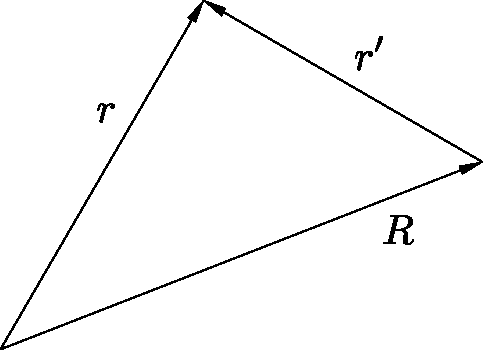
\includegraphics[width=0.3\textwidth]{images/fig_sist_part.pdf}	 
	\end{center}
	\caption{Sistema de partículas}
\end{figure} 

% =================================================================================================
\section{Trabajo en un sistema de partículas}
% =================================================================================================

Empezamos desde
\[
W = W^{ext} + W^{int}
\]
donde el trabajo externo puede escribirse
\notamargen{Quiero un $\ell$ en bold, no me gusta el ${\bf s}$.}
\be
W^{ext} = \sum_i^N \int_1^2 \vb{F}_i^e \cdot d\vb{s}
\label{mc_work_ext}
\ee

La no dependencia del camino para la integral que da \eqref{mc_work_ext} requiere que 
\[
\vb{F}_i^e = \vb{F}_i^e( \vb{r}_i ) \qquad \nabla_{r_i} \times \vb{F}_i^e = 0
\]
y entonces puedo inducir la existencia de una función potencial para las fuerzas externas,
\notamargen{barra resizeable ya.}
\[
W^{ext} = - \sum_i^N  \left. \Delta V_i \right]_1^2 
\]

Por otro lado,
\[
W^{int}_c = \int_1^2 \sum_{\substack{j\\j\neq i}}^N  \vb{F}_{ij}^e \cdot d\vb{s}_i  
\]
\[
\sum_i^N W_i^{int} =  W^{int} = \sum_{\substack{j \\ i\neq j}}^N  \int_1^2 \sum_{\substack{j \\ j\neq i}}^N  \vb{F}_{ij}^e \cdot 
d\vb{s}_i  
\]

% =================================================================================================
\section{Lagrangiano cíclico en el tiempo}
% =================================================================================================

Empecemos desde la derivada total con respecto al tiempo del lagrangiano,
\[
\frac{d}{dt}\left( \Lag( q, \dot{q}, t)\right) = \dpar{\Lag}{q} \dot{q} + \dpar{\Lag}{\dot{q}} \ddot{q} + \dpar{\Lag}{t}
\]
y usando la derivada total del término 
\[
\frac{d}{dt}\left( \dpar{\Lag}{\dot{q}}\dot{q}\right) =
\frac{d}{dt}\left( \dpar{\Lag}{\dot{q}} \right) \dot{q} + \dpar{\Lag}{\dot{q}} \ddot{q} .
\]

Reemplazando una en otra resulta que 
\[
\frac{d}{dt}\left( \Lag( q, \dot{q}, t)\right) = \dpar{\Lag}{q} \dot{q} + \frac{d}{dt}\left( \dpar{\Lag}{\dot{q}}\dot{q}\right) -
\frac{d}{dt}\left( \dpar{\Lag}{\dot{q}} \right) \dot{q} + \dpar{\Lag}{t}
\]
y acomodando un poco
\[
\frac{d}{dt}\left( \Lag( q, \dot{q}, t)\right) = 
\left[ \dpar{\Lag}{q}  - \frac{d}{dt}\left( \dpar{\Lag}{\dot{q}} \right) \right] \dot{q} + 
\frac{d}{dt}\left( \dpar{\Lag}{\dot{q}}\dot{q}\right)  + \dpar{\Lag}{t}
\]
\[
\frac{d}{dt}\left( \Lag( q, \dot{q}, t)\right) = \frac{d}{dt}\left( p \dot{q} \right) + \dpar{\Lag}{t}
\]
y entonces previo pase mágico de términos,
\[
\frac{d}{dt}\left( p\dot{q} - \Lag \right) = -\dpar{\Lag}{t}
\]
y si definimos
\[
\Ham \equiv p\dot{q} - \Lag 
\]
resulta que 
\[
\dtot{\Ham}{t} = - \dpar{\Lag}{t}.
\]

Entonces si el lagrangiano no depende explícitamente del tiempo se tiene que $\Ham = cte.$. Además,
si se cumplen 
\[
T=T_2 \qquad V \neq V(\dot{q})
\]
y además los vínculos no dependen del tiempo se tiene que $\Ham=E$, es decir, el Hamiltoniano es la
energía. La condicion de que los vínculos no dependan del tiempo genera en realidad que $T=T_2$.

Por otro lado $E = cte.$ si $W^{nc} = 0$.

% =================================================================================================
\section{Energía cinética y el hamiltoniano}
% =================================================================================================

Dado que la energía cinética tiene la forma general
\[
T = \underbrace{\frac{1}{2} \sum_i^N m_i \left( \dpar{\vb{r}_i}{t} \right)^2}_{T_0}  +
\underbrace{\sum_j^{3n-k} b_j(q_1,...,q_{3N-k},t)\dot{q}_j  }_{T_1} +
\underbrace{\frac{1}{2} \sum_j^{3n-k}\sum_s^{3n-k}  a_{js}(q_1,...,q_{3N-k},t)\dot{q}_s\dot{q}_j }_{T_2}
\]
entonces se sigue que 
\be
E = T_0 + T_1 + T_2 + V
\label{mc_E}
\ee
y como 
\[
p_i = \dpar{\Lag}{\dot{q}_i} = T_1 + 2T_2 
\]
es 
\[
\Ham = \sum_i^N p_i\dot{q}_i - (T_0 + T_1 + T_2 - V) = 2T_2 + T_1 - T_0 - T_1 - T_2 + V = T_2 - T_0 + V
\]
pero como E es \eqref{mc_E} se tendrá 
\[
E = H \iff 2T_0 + T1 = 0
\]
y un solución de este sistema es, por supuesto, $T_0 = T_1 = 0$

% =================================================================================================
\section{Principio de acción mínima}
% =================================================================================================

También Principio variacional de Hamilton. Partimos de una acción,
\[
S = \int_{t_i}^{t_f} \Lag( q_i, \dot{q}_i, t ) dt \qquad \Lag = T-V
\]

La trayectoria real de un sistema con lagrangiano $\Lag$ es tal que $S$ es mínimo para cualquier 
trayectoria posible entre $q(t=t_i)$ y $q(t=t_f)$. Consideramos una variación con extremos fijos,
es decir 
\[
\delta q(t=t_i) = 0 \qquad \delta q(t=t_f) = 0
\]
y a tiempo fijo $\delta t = 0$. Esto último signfica que todas las trayectorias emplearán el 
mismo tiempo (no se variará).
\notamargen{Cuán sketchi es todo esto!! Mucho para aclarar. Tal vez se justifique un minicurso
de variacional como apéndice.}

\begin{figure}
	\begin{center}
	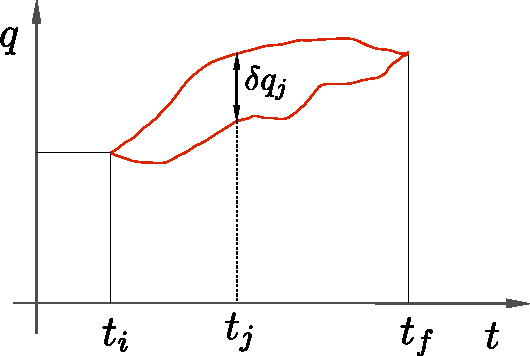
\includegraphics[width=0.4\textwidth]{images/fig_accion.pdf}	 
	\end{center}
	\caption{El principio de acción mínima}
\end{figure}

Consideramos una variación de la integral,
\[
\delta I =  \int_{t_i}^{t_f} \sum_i^N \left( \dpar{\Lag}{\dot{q}_i} \delta \dot{q}_i + \dpar{\Lag}{q_i} \delta q_i  \right) dt,
\]
y notamos que será beneficioso utilizar integración por partes para expresar todo en función de
las variaciones de las coordenadas (las $\delta q_i$), de manera que como
\[
\frac{d}{dt}\left( \dpar{\Lag}{\dot{q}_i} \delta q_i \right) =
\frac{d}{dt}\left( \dpar{\Lag}{\dot{q}_i} \right) \delta q_i + \dpar{\Lag}{\dot{q}_i}\delta \dot{q}_i,
\]
resulta
\[
\delta I =  \int_{t_i}^{t_f} \sum_i^N \left[ \frac{d}{dt}\left( \dpar{\Lag}{\dot{q}_i} \delta q_i \right) -
\frac{d}{dt}\left( \dpar{\Lag}{\dot{q}_i} \right) \delta q_i + \dpar{\Lag}{q_i} \delta q_i  \right] dt,
\]
separamos los dos términos,
\[
\delta I =  \int_{t_i}^{t_f} \sum_i^N \left[ \frac{d}{dt}\left( \dpar{\Lag}{\dot{q}_i} \delta q_i \right) \right] dt -
\int_{t_i}^{t_f} \sum_i^N \left[ \frac{d}{dt}\left( \dpar{\Lag}{\dot{q}_i} \right) - \dpar{\Lag}{q_i} 
\right]  \delta q_i  dt,
\]
y resulta que el primero por el teorema fundamental del cálculo es
\be
\int_{t_i}^{t_f} \sum_i^N \left[ \frac{d}{dt}\left( \dpar{\Lag}{\dot{q}_i} \delta q_i \right) \right] dt =
\left. \dpar{\Lag}{\dot{q}_i} \delta q_i\right|_{t_i}^{t_f}
\label{mc_borde_term}
\ee
y es nulo porque $\delta q_i=0$ en los extremos (recordemos que las variaciones son nulas en los extremos de
integración). Decimos que este es un término de superficie.
Entonces
\[
\delta I =  -\int_{t_i}^{t_f} \sum_i^N \left[ \frac{d}{dt}\left( \dpar{\Lag}{\dot{q}_i} \right) - \dpar{\Lag}{q_i} 
\right]  \delta q_i  dt = 0
\]
se verificará por el cumplimiento de las ecuaciones de Euler-Lagrange
\[
\sum_i^N  \left[ \frac{d}{dt}\left( \dpar{\Lag}{\dot{q}_i} \right) - \dpar{\Lag}{q_i} \right] = 0.
\]

Luego, si se hace $\Lag' = \Lag + df/dt$ (ambos lagrangianos difieren en una derivada total con 
respecto al tiempo) la trayectoria que minimiza $\Lag'$ es la que misma que minimiza
$\Lag$ por la condición dada por \eqref{mc_borde_term}. Entonces 
\[
\delta S = 0 \iff \sum_i^N  \left[ \frac{d}{dt}\left( \dpar{\Lag}{\dot{q}_i} \right) - \dpar{\Lag}{q_i} \right] = 0.
\]

La moraleja es que si los lagrangianos difieren en una derivada total del tiempo obtenemos la misma
física.

% =================================================================================================
\section{Aplicaciones del principio de acción mínima}
% =================================================================================================

\[
S = \int (T-V_0) dt
\]
donde el lagrangiano es con $V=V_0$ constante (un lagrangiano sujeto a potencial constante).
La integral de acción da una medida de la longitud de la órbita (el espacio recorrido).
Para una partícula sujeta a $V=0$
\[
S = \frac{1}{2}\int m v_0^2 dt = \frac{1}{2}mv_0^2(t-t_0)
\]
de manera que $v_0(t-t_0)$ representa la distancia $d$ recorrida, y es 
\[
S = \frac{1}{2}mv_0 d
\]

Comentario sobre el cálculo de las variaciones
\notamargen{Esta idea debe estar en el suplemento matemático que le dedicaremos a variacional}
\[
I = \int f\left(x, \dtot{x}{t}, t\right) dt 
\]
entonces $I$ es extremo si
\[
\frac{d}{dt} \left( \dpar{f}{[dx/dt]}\right) - \dpar{f}{x} = 0
\]
También podemos encontrar esta notación, dependiendo del tipo de problema,
\[
I = \int f\left(y, \dtot{y}{x}, x\right) dx 
\]


% =================================================================================================
\section{Multiplicadores de Lagrange}
% =================================================================================================

Partimos de la acción
\[
S = \int_{t_i}^{t_f} \Lag \left( q_i[t], \dot{q}_i[t], t \right) dt
\]
entonces 
\[
\delta S = 0 \quad \Leftrightarrow \quad \int
\sum_{j=1}^{N} \left[ \frac{d}{dt}\left( \dpar{\Lag}{\dot{q}_j} \right) -\dpar{\Lag}{q_j} \right]\delta q_j dt
\]
donde $\delta q_j$ son desplazamientos independientes. Si no se pued despejar alguna $\delta q_j$ (con 
vínculos no-holónomos, por ejemplo) entonces algún $\delta q_j$ es independiente de modo que para que 
valga $\delta S =0 $ necesitaré 
\[
\sum_{\ell}^N a_\ell^k(q_i,t) \dot{q}_\ell + b^k(q_i,t) = 0
\]
que son los vínculos ($k=1,...,s$); son $s$ ecuaciones de vínculo.
Multiplicamos por $\delta t$ y vemos que no son independientes
\[
\sum_{\ell}^N a_\ell^k(q_i,t) \delta {q}_\ell + b^k(q_i,t) \delta t= 0
\]

Sean $\delta q_\ell$ variación a $t$ fijo, entonces 
\[
\sum_{\ell}^N a_\ell^k(q_i,t) \delta {q}_\ell
\]
\[
\int_{t_i}^{t_f} \lambda^k \sum_{\ell}^N a_\ell^k(q_i,t) \delta {q}_\ell dt = 0
\]
recordando que $\ell$ suma en los grados de libertad. Podemos sacar la suma fuera,
\[
\sum_{k}^s \int_{t_i}^{t_f} \lambda^k \sum_{\ell}^N a_\ell^k(q_i,t) \delta {q}_\ell dt = 0
\]
Absorbo la otra sumatoria en el segundo término y paso de $\ell \to j$.
\[
\int  \sum_{j=1}^N \left\{ \frac{d}{dt}\left( \dpar{\Lag}{\dot{q}_j} \right) -\dpar{\Lag}{q_j}
- \sum_{k}^s \lambda^k a_\ell^k(q_i,t) \right\} \delta {q}_\ell dt = 0
\]
entonces 
\[
\sum_{j=1}^N \frac{d}{dt}\left( \dpar{\Lag}{\dot{q}_j} \right) -\dpar{\Lag}{q_j} =
\sum_{j=1}^N \sum_{k}^s \lambda^k a_\ell^k(q_i,t) =  
\sum_{j=1}^N \sum_{k}^s \lambda^k \nabla_j f^k \cdot \frac{\delta \vb{r}_j}{\delta q_j} 
\]
siendo $\nabla_j f^k $ el gradiente de la ecuación de víngulo respeco de $j$ y donde $\lambda^k$
es la fuerza de vínculo asociada al vínculo no despejado pues como la fuerza generalizada
(que no proviene de potencial)
\[
Q_j = \sum_i^N \vb{F}_i^a \cdot \dpar{\vb{r}_i}{q_j}
\]
y comparando vemos que 
\[
Q_j = \sum \lambda^k a^k_j(q_j,t) \quad \textrm{vínculos no holónomos}
\]
\[
Q_j=  \sum \lambda^k \nabla_j f^k \cdot \delta \vb{r}_j  \quad \textrm{vínculos holónomos}
\]

En el caso de vínculos holónomos 
\[
g(\vb{r}_1,...,\vb{r}_n,t) = 0 
\]
donde no quise despejar en función de $q_q,...,q_n$ resulta que 
\notamargen{El supraíndice con $\delta q_j$ va sobre el igual en realidad.}
\[
Q_j^{\delta q_j} =  \sum_i^N \lambda (\nabla_i f^k\cdot\delta\vb{r}_i)
\]
donde $\delta\vb{r}_i$ es un desplazamiento virtual de la partícula.
Vamos a reescribir este término,
\[
\sum_i^N \dpar{g^k}{\vb{r}_i} \delta \vb{r}_i = 0
\]
\[
\nabla_i f^k\cdot\delta\vb{r}_i = \sum_i \dpar{g^k}{\vb{r}_i} \dpar{\vb{r}_i}{q_j} \delta q_j
\]
\[
Q_j^{\delta q_j} =  \lambda \sum_k \dpar{g^k}{\vb{r}_i} \sum_j \dpar{\vb{r}_i}{q_j} \delta q_j
\]
luego como 
\[
a^k_j \equiv \dpar{g^k}{\vb{r}_i}
\]
se sigue que los $\lambda^k$ son las fuerzas de vínculo.

En el caso de vínculos no holónomos $\lambda^k$ son las fuerzas de vínculo asociadas a los 
vínculos no retirados.

\[
Q_j {\delta q_j} =  \sum \lambda^k (\nabla_i g^k\cdot\delta\vb{r}_i)
\]
\[
Q_j =  \sum_k \lambda^k \dpar{g^k}{\vb{r}_i} \dpar{\vb{r}_i}{q_j}
\]
\[
Q_j =  \sum_k \lambda^k \dpar{g^k}{q_j}
\]
entonces $\lambda^k=F^v$.

Como extra escribamos que para cada grado de libertad $j$ 
\[
\dpar{\Lag}{q_j} - \frac{d}{dt}\left( \dpar{\Lag}{\dot{q}_j} \right) - \sum_k^s \lambda^k a_j^k \equiv 0
\]
donde $\delta q_j$ son ahora independientes.
\[
Q_j = \sum_i^N F_i^a \dpar{\vb{r}_i}{q_j}. 
\]

% =================================================================================================
\section{Constantes de movimiento y simetrías}
% =================================================================================================

Sean 
\[
\frac{d}{dt}\left( \dpar{\Lag}{\dot{q}_j} \right) - \dpar{\Lag}{q_j}  = 0 
\]
si
\[
 \dpar{\Lag}{q_j}  = 0 
\]
entonces 
\[
\frac{d}{dt}\left( \dpar{\Lag}{\dot{q}_j} \right) = 0
\]
y se ve que 
\[
\dpar{\Lag}{\dot{q}_j} \equiv p_i = cte.
\]

Si $\delta q_i$ es traslación rígida entonces $p_i = \vb{P}\cdot\hat{n}$ y $Q_j= \vb{F}\cdot\hat{n}$ en
cambio si es rotación rígida se tiene $p_i = \vb{L}\cdot\hat{n}$ y $Q_j= \vb{\Tau}\cdot\hat{n}$.
De tal forma vale que 
\[
\dpar{T}{q_i} = 0
\]
pués $T$ es escalar y no cambia ante una rotación y $T=T(\dot{q})$ no depende explícitamente de las
coordenadas (no depende del origen decía ¿?). Luego $T=T_2$ y
\[
\dpar{\Lag}{q_i} = 0 = \dpar{T}{q_i} - \dpar{V}{q_i} = 0
\]
Como $V \neq V(\dot{q})$ entonces las ecuaciones de Euler-Lagrange adoptan la forma
\[
\frac{d}{dt}\left( \dpar{T}{\dot{q}_j} \right) + \dpar{V}{q_j}  = 0 
\]
\[
\frac{d}{dt}\left( \dpar{T}{\dot{q}_j} \right) = - \dpar{V}{q_j}   
\]
\[
\frac{d}{dt}\left( p_j \right) = - \dpar{V}{q_j}   
\]
y entonces 
\[
\dot{p}_j = -\dpar{V}{q_j}   
\]
es la fuerza total proyectada en $\hat{n}$.

% =================================================================================================
\section{El teorema de Noether}
% =================================================================================================

Si existe una transformación continua $q_i \longrightarrow q_i + \delta q_i$ que deje invariante el
$\Lag$ entonces hay una constante de movimiento asociada a dicha transformación.

La transformación es 
\[
q_i \longrightarrow q_i' = q_i + \delta q_i
\]
y cumple 
\[
\Lag(q_i, \dot{q}_i , t) = \Lag(q_i', \dot{q}_i' , t) =
\Lag(q_i[q_i',t], \dot{q}_i[\dot{q}_i',t] , t)
\]
y así si consideramos una variación a $t$ fijo,
\[
\delta \Lag = \sum_i 
\]












% ============================================================================


\bibliographystyle{CBFT-apa-good}	% (uses file "apa-good.bst")
\bibliography{CBFT.Referencias} % La base de datos bibliográfica

\end{document}

	
		\documentclass[10pt,oneside]{CBFT_book}
	% Algunos paquetes
	\usepackage{amssymb}
	\usepackage{amsmath}
	\usepackage{graphicx}
	\usepackage{libertine}
	\usepackage[bold-style=TeX]{unicode-math}
	\usepackage{lipsum}

	\usepackage{natbib}
	\setcitestyle{square}

	\usepackage{polyglossia}
	\setdefaultlanguage{spanish}


	\usepackage{CBFT.estilo} % Cargo la hoja de estilo

	% Tipografías
	% \setromanfont[Mapping=tex-text]{Linux Libertine O}
	% \setsansfont[Mapping=tex-text]{DejaVu Sans}
	% \setmonofont[Mapping=tex-text]{DejaVu Sans Mono}

	%===================================================================
	%	DOCUMENTO PROPIAMENTE DICHO
	%===================================================================

% \title{CBFT Mecánica clásica}
% \author{Simetrías}
% \date{\today}

\begin{document}
% \maketitle
% \tableofcontents
\chapter{Simetrías}

% =================================================================================================
\section{Constantes de movimiento y simetrías}
% =================================================================================================

Sean 
\[
	\frac{d}{dt}\left( \dpar{\Lag}{\dot{q}_j} \right) - \dpar{\Lag}{q_j}  = 0 
\]
si
\[
	\dpar{\Lag}{q_j}  = 0 
\]
entonces 
\[
	\frac{d}{dt}\left( \dpar{\Lag}{\dot{q}_j} \right) = 0
\]
y se ve que 
\[
	\dpar{\Lag}{\dot{q}_j} \equiv p_i = cte.
\]

Si $\delta q_i$ es traslación rígida entonces $p_i = \vb{P}\cdot\hat{n}$ y $Q_j= \vb{F}\cdot\hat{n}$ en
cambio si es rotación rígida se tiene $p_i = \vb{L}\cdot\hat{n}$ y $Q_j= \vb{\Tau}\cdot\hat{n}$.
De tal forma vale que 
\[
	\dpar{T}{q_i} = 0
\]
pués $T$ es escalar y no cambia ante una rotación y $T=T(\dot{q})$ no depende explícitamente de las
coordenadas (no depende del origen decía ¿?). Luego $T=T_2$ y
\[
	\dpar{\Lag}{q_i} = 0 = \dpar{T}{q_i} - \dpar{V}{q_i} = 0
\]
Como $V \neq V(\dot{q})$ entonces las ecuaciones de Euler-Lagrange adoptan la forma
\[
	\frac{d}{dt}\left( \dpar{T}{\dot{q}_j} \right) + \dpar{V}{q_j}  = 0 
\]
\[
	\frac{d}{dt}\left( \dpar{T}{\dot{q}_j} \right) = - \dpar{V}{q_j}   
\]
\[
	\frac{d}{dt}\left( p_j \right) = - \dpar{V}{q_j}   
\]
y entonces 
\[
	\dot{p}_j = -\dpar{V}{q_j}   
\]
es la fuerza total proyectada en $\hat{n}$.

% =================================================================================================
\section{El teorema de Noether}
% =================================================================================================

Si existe una transformación continua $q_i \longrightarrow q_i + \delta q_i$ que deje invariante el
$\Lag$ entonces hay una constante de movimiento asociada a dicha transformación.

La transformación es 
\[
	q_i \longrightarrow q_i' = q_i + \delta q_i
\]
y cumple 
\[
	\Lag(q_i, \dot{q}_i , t) = \Lag(q_i', \dot{q}_i' , t) =
	\Lag(q_i[q_i',t], \dot{q}_i[\dot{q}_i',t] , t)
\]
y así si consideramos una variación a $t$ fijo,
\[
	\delta \Lag = \sum_i \dpar{\Lag}{q_i}\delta q_i + \dpar{\Lag}{\dot{q}_i}\delta \dot{q}_i =
	\sum_i \dpar{\Lag}{q_i}\delta q_i + \frac{d}{dt}\left( \dpar{\Lag}{\dot{q}_i}\delta q_i \right)
	- \frac{d}{dt}\left( \dpar{\Lag}{\dot{q}_i} \right) \delta q_i = 0
\]
\[
	\delta \Lag = \sum_i \left[ \dpar{\Lag}{q_i} - \frac{d}{dt}\left( \dpar{\Lag}{\dot{q}_i} \right) \right]
	\delta q_i + \frac{d}{dt}\left( \dpar{\Lag}{\dot{q}_i}\delta q_i \right) = 0
\]
pero como el primer término del RHS es nulo por las ecuaciones de Euler-Lagrange tenemos que 
\[
	\delta \Lag = \frac{d}{dt}\left( \sum_i \dpar{\Lag}{\dot{q}_i}\delta q_i \right)  = 0,
\]
lo que está dentro del paréntesis es la cantidad conservada. 
Recordemos que 
\[
	\delta q_i = q'_i - q_i 
\]
y una traslación infinitesimal es 
\[
	\vb{r}_i' - \vb{r}_i = \delta \vb{r}. 
\]

La variable cíclica es un caso particular de teorema de Noether, pero hay constantes de movimiento que 
no provienen de ninguna simetría.
\[
	\frac{d}{dt}\left( \sum_i \dpar{\Lag}{\dot{q}_i} ( \delta \alpha \hat{n}\times \vb{r}_i ) \right) 
\]
\[
	\frac{d}{dt}\left( \delta\alpha \sum_i \vb{p}_i \times \vb{r}_i  \right) =
	\delta\alpha \frac{d}{dt}\left(  \sum_i \vb{p}_i \times \vb{r}_i  \right) = 0
\]
siendo $\delta \alpha \equiv \epsilon$ un parámetro infinitesimal.
Para $k$ grados de libertad
\begin{align*}
	q'_i &= q_i + \underbrace{\epsilon_i g_i(q_1,...,q_n,t)}_{\delta q} \\
	... \\
	q'_k &= ...
\end{align*}
\[
	\vb{r}_i' = \vb{r}_i + \delta\vb{r} \quad \textrm{traslación rígida}
\]
\[
	\vb{r}_i' = \vb{r}_i + \delta\alpha \; \hat{n}\times\vb{r}_i \quad \textrm{rotación rígida}
\]
o también 
\[
	\delta \vb{r} \times \vb{r}
\]

$T$ es invariante siempre frente a (por ser un escalar)
\[
	T = T' 
\]
entonces habrá que examinarlo.
Constatemos que 
\[
	V = V(|\vb{r}_i - \vb{r}_j|)
\]
es invariancia ante una traslación rígida, y
\[
	V = V(x_1,x_2)
\]
es una invariancia de traslación en $x_3$.

$\Lag$ tendrá como constante un momento lineal si $V$ es invariante frente a traslación.
$\Lag$ tendrá como constante un momento angular si $V$ es invariante frente a rotación.
$\Lag$ tendrá como constante una combinación si $V$ es invariante frente a una roto-traslación.

Otra construcción posible es 
\[
	\delta \Lag = 0
\]
\[
	\Lag( q_i , \dot{q}_i, t ) - \Lag(q_i' , \dot{q}_i' , t) = 0 
\]
pidiendo que $d\Lag = 0$ llego a 
\[
	\sum \left\{ \frac{d}{dt}\left( \dpar{\Lag}{\dot{q}_i} \delta q \right) - 
	\frac{d}{dt}\left( \dpar{\Lag}{\dot{q'}_i} \delta q' \right)  \right\} = 0
\]
\notamargen{Las primas están mal. Hay que pensar una construcción adecuada.
Queda odd.}
\[
	\sum \left\{ \frac{d}{dt}\left( \dpar{\Lag}{\dot{q}_i} \delta q \right) - 
	\frac{d}{dt}\left( \dpar{\Lag}{\dot{q'}_i} \delta q \right) -
	\frac{d}{dt}\left( \dpar{\Lag}{\dot{q'}_i} \sum_\ell^s \epsilon_\ell g_i^\ell \right) \right\} = 0
\]
y podemos usar que 
\[
	\dpar{\Lag}{\dot{q'}_i} = \dpar{\Lag}{\dot{q}_i}
\]
pues $g\neq g(t)$ y es todo a tiempo fijo. Se tiene 
\[
	q' = q + \delta q
\]
\[
	q_i' = q_i + \sum_\ell^s \epsilon_\ell g_i^\ell
\]
siendo esta la transformación general
\[
	\delta q_i' = \delta q_i + \sum_\ell^s \epsilon_\ell g_i^\ell
\]

Extraemos también que 
\[
	\dpar{\Lag}{\dot{q'}_i} \sum_\ell^s \epsilon_\ell g_i^\ell = C
\]

Se puede pensar también como que $\Lag$ es invariante ante la transformación infinitesimal
$\delta q$
\[
	\delta\Lag = 0 = \sum_i^N \dpar{\Lag}{q_i}\delta q_i + \dpar{\Lag}{\dot{q}_i}\delta \dot{q}_i
\]
\[
	\delta\Lag = 0 = \sum_i^N \left[ \dpar{\Lag}{q_i} - \frac{d}{dt}\left( \dpar{\Lag}{\dot{q}_i} \right)
	\right]\delta q_i  + \sum_i^N \frac{d}{dt}\left( \dpar{\Lag}{\dot{q}_i} \delta q_i \right)  = 0
\]
siendo el primer término nulo, y siendo lo que se conserva lo que aparece en el segundo término,
donde 
\[
	\delta q_i =  \sum_\ell^s \epsilon_\ell g_i^\ell(q_1,q_2,...,q_n)
\]
Finalmente 
\[
	\delta \Lag = 0 = \frac{d}{dt}\left( \sum_i^N \dpar{\Lag}{\dot{q}_i} \delta q_i \right) 
\]


% =================================================================================================


% \bibliographystyle{CBFT-apa-good}	% (uses file "apa-good.bst")
% \bibliography{CBFT.Referencias} % La base de datos bibliográfica

\end{document}

	
		\documentclass[10pt,oneside]{CBFT_article}
	% Algunos paquetes
	\usepackage{amssymb}
	\usepackage{amsmath}
	\usepackage{graphicx}
	\usepackage{libertine}
	\usepackage[bold-style=TeX]{unicode-math}
	\usepackage{lipsum}

	\usepackage{natbib}
	\setcitestyle{square}

	\usepackage{polyglossia}
	\setdefaultlanguage{spanish}


	\usepackage{CBFT.estilo} % Cargo la hoja de estilo

	% Tipografías
	% \setromanfont[Mapping=tex-text]{Linux Libertine O}
	% \setsansfont[Mapping=tex-text]{DejaVu Sans}
	% \setmonofont[Mapping=tex-text]{DejaVu Sans Mono}

	%===================================================================
	%	DOCUMENTO PROPIAMENTE DICHO
	%===================================================================

\title{CBFT Mecánica clásica}
\author{Fuerzas centrales}
\date{\today}

\begin{document}
\maketitle
\tableofcontents

% =================================================================================================
\section{Fuerzas centrales}
% =================================================================================================

Una fuerza central es aquella que cumple
\[
	\vb{F}(r) = f(r)\hat{r} = - \dpar{V}{r}
\]
de tal suerte que la parte cinética del lagrangiano es 
\[
	\Lag = \frac{1}{2}m \left( \dot{r}^2 + r^2 \dot{\theta}^2 + r^2 \sin(\theta)^2\dot{\phi}^2 \right)
\]

El momento angular $\vb{L}$ se conserva puesto que $\vb{\tau} = \vb{r} \times \vb{F}=0$. Como es 
$\vb{L} = \vb{r} \times \vb{p} = \vb{r} \times m\dot{\vb{r}} = cte$ entonces se sigue que $\vb{r},\vb{p}$
se hallan contenidos en el mismo plano.

Puedo pedir, sin pérdida de generalidad, que $\theta=\pi/2$ y entonces 
\[
	\Lag = \frac{1}{2}m \left( \dot{r}^2 + r^2 \dot{\theta}^2 \right) - V(r).
\]

Como $\phi$ es cíclica se tiene
\[
	\dpar{\Lag}{\dot{\phi}} = L = mr^2\dot{\phi}
\]
que no es otra cosa que la conservación del momento angular, información que puede ser llevada al
lagrangiano,
\[
	\Lag = \frac{1}{2}m \dot{r}^2 + \left[ \frac{L^2}{2 m r^2} - V(r) \right]
\]
donde el último corchete será lo que llamaremos un potencial efectivo $V_{eff}$,
\[
	\Lag = \frac{1}{2}m \dot{r}^2 + V_{eff}(r)
\]

La ecuación de Euler-Lagrange resulta en
\[
	m\ddot{r} - \frac{L^2}{mr^3} + \dpar{V}{r} = 0
\]
pero es más sencillo utilizar la conservación de la energía que explícitamente tiene la expresión
\[
	E = \frac{1}{2}m \dot{r}^2 + \frac{L^2}{2 m r^2} + V(r)
\]
desde la cual se puede integrar directamente la trayectoria $r=r(t)$ según
\[
	\dtot{r}{t} = \sqrt{ \frac{2}{m}\left( E - \frac{L^2}{2 m r^2} - V(r) \right)},
\]
aunque suele ser más útil la trayectoria en el espacio físico $r=r(\phi)$ o bien $\phi=\phi(r)$.
\[
	m r^2 \dtot{\phi}{t} = L \quad \longrightarrow m r^2 \dtot{\phi}{r} \dot{r} = L
\]
luego
\[
	\dot{r} d\phi = \frac{L}{m r^2} dr
\]
\[
	\int d\phi = \int \frac{L/mr^2}{\sqrt{ \frac{2}{m}\left( E - \frac{L^2}{2 m r^2} - V(r) \right)}}dr
\]

En el gráfico bajo estas líneas ilustramos muchas de las características de la física del problema
de fuerzas centrales.

% =================================================================================================
\section{Solución a partir de las ecuaciones de Euler-Lagrange}
% =================================================================================================

\[
	m \ddot{r} -\frac{L^2}{m r^3} -\dpar{V}{r}= 0 
\]
\[
	d \phi = \frac{L}{m r^2} dt \qquad \longrightarrow \quad  \dpar{\phi}{r}\dpar{r}{t}  = \frac{L}{m r^2}
\]
\[
	\frac{d}{t}(\dot{r}) = \frac{L}{m r^2} \frac{d}{\phi}(\dot{r})
\]
\[
	m \dtot[2]{r}{t} -\frac{L^2}{m r^3} = -\dpar{V}{r}
\]
\[
	\frac{L}{r^2} \frac{d}{\phi}\left( \dtot{r}{t} \right) -\frac{L^2}{m r^3} = -\dtot{V}{r}
\]
\[
	\frac{L}{r^2} \frac{d}{\phi}\left( \frac{L}{m r^2}\dtot{r}{\phi} \right) -\frac{L^2}{m r^3} = -\dtot{V}{r}
\]
y acá probamos el conveniente cambio de variables
\[
	U = \frac{1}{r} \qquad dU = -\frac{1}{r^2} dr 
	\qquad \dtot{U}{\phi} = -\frac{1}{r^2}\dtot{r}{\phi} = -U^2\dtot{r}{\phi}
\]
\[
	U^2 L \frac{d}{d\phi} \left\{ -\frac{L}{m}\dtot{U}{\phi} \right\} - \frac{L^2}{m r^3} U^3 = F(1/U)
\]
\[
	- \frac{U^2 L^2}{m} \dtot[2]{U}{\phi} - \frac{L^2}{m r^3} U^3 = F(1/U)
\]
\[
	- \frac{U^2 L^2}{m} \left[ \dtot[2]{U}{\phi} + U \right] = F(1/U)
\]
o bien 
\[
	\left[ \dtot[2]{U}{\phi} + U \right] = - \frac{F(1/U) m}{U^2 L^2}. 
\]

En el caso del potencial de Kepler será 
\[
	\left[ \dtot[2]{U}{\phi} + U \right] = - \frac{K m}{L^2},
\]
es decir que el miembro derecho es una constante. Sale fácil entonces.

% =================================================================================================
\section{Velocidad areolar}
% =================================================================================================

\[
	\dot{\phi} = \frac{L}{m r^2}
\]

De la figura puede verse que 
\[
	A = \frac{1}{2} r^2 d\phi 
\]
y  entonces
\[
	\dtot{A}{t} = \frac{1}{2} r^2 \dtot{\phi}{t} = \frac{1}{2} r^2 \dot{\phi} = \frac{1}{2}\frac{L}{m} = cte.
\]

% =================================================================================================
\section{Las fuerzas centrales y las leyes de Kepler}
% =================================================================================================

Tenemos 
\[
	\int d\phi = \int \frac{(L/Mr^2)}{\sqrt{ \frac{2}{m}(E - V_{eff})}} dr	\qquad
	\dtot[2]{U}{\phi} + U  = - \frac{F(1/U) m}{U^2 L^2} \quad U = 1/r
\]
que es simétrica respecto a $\phi$ y $-\phi$. Esto determina una simetría orbital si
tomamos
\[
	U(\phi=0) = U_0 	\qquad		\left. \dtot{U}{\phi} \right|_{\phi=0}= 0
\]
lo cual significa que $U_0$ es un extremo (punto apsidal).

Calculemos ahora el ángulo que recorre una oscilación completa,
\[
	\Delta \phi = 2\int_{r_m}^{r_M} \frac{(L/Mr^2)}{\sqrt{ \frac{2}{m}(E - V_{eff})}} dr
\]

Si $\Delta \phi = 2 q $ siendo $q= (m/n)\pi $ son $m,n \in \mathbb{Z}$ entonces
\[
	\Delta \phi = 2 \frac{m}{n} \pi 
\]
\[
	\frac{m}{n} = \frac{2\pi}{\Delta \phi}
\]
y esto significaría que la órbita se cierra.

La ecuación a resolver es 
\[
	\dtot[2]{U}{\phi} + \left( U  - \frac{k m}{L^2} \right) = 0
\]
o bien 
\[
	\dtot[2]{\beta}{\phi} + \beta = 0
\]
entonces
\[
	\beta = A \cos( \phi -\phi_0 )
\]
\[
	U = \frac{km}{L^2} +  A \cos( \phi -\phi_0 )
\]
\[
	\frac{1}{r} = \frac{km}{L^2} +  A \cos( \phi -\phi_0 )
\]
y habría que usar $r_m, r_M$ para evaluar $A$.


Con respecto a las elipses
\[
	\frac{x^2}{a^2} + \frac{y^2}{b^2} = 1	\qquad \sigma^2 = a^2 - b^2
\]
\[
	b = a \sqrt{ 1 - (\sigma/a)^2 }
\]

Por otro lado,
\[
	s^2 = (2\sigma)^2 + r^2 - 4\sigma r \cos( \pi - \phi )
\]
\[
	( 2a -r )^2 = 4\sigma^2 + r^2 + 4\sigma r \cos(\phi)
\]
y definiendo $ \sigma/a \equiv \varepsilon$ resulta
\[
	a - r = \varepsilon ( \sigma + r\cos(\phi) )
\]
y esto es una elipse.
\notamargen{Acá hay que hacer un laburo muy importante.}

Entonces en resumen, las leyes de Kepler son
\begin{enumerate}
 \item Los planetas giran en órbitas elípticas con el Sol en uno de sus focos. Esto es común de los potenciales del tipo 
	\[
		V \propto 1/r
	\]
 \item El radio vector recorre áreas iguales en tiempos iguales
	\[
		A = \frac{1}{2} r^2 d\phi \quad \longrightarrow \dtot{A}{t} = \frac{r^2}{2} \dot{\phi} = \frac{L}{2m} (cte.)
	\]
 \item 
 \[
	\dtot{A}{t} = \frac{L}{2m}
 \]
 \[
	\pi a b = \int dA = \frac{L}{2m} \int dt = \frac{L}{2m} \tau \qquad a = \frac{L\tau}{2\pi m b} 
 \]
 pero como $km/L^2 = a/b^2$ es
 \[
	B = L \sqrt{\frac{a}{k m}}
 \]
 \[
	a^3 = \frac{GM}{4\pi^2} \tau^2
 \]
 y esto es independiente de la masa del planeta.
 
 Trabajamos más con la elipse,
 \[
	r_M + r_m = 2a
 \]
 \[
	E = \frac{L^2}{2mr^2} - \frac{k}{r}	\qquad\qquad E - \frac{L^2}{2m} U^2 - kU = 0
 \]
 \[
	\frac{1}{r_{m,M}} = \frac{ \frac{2mkE}{L^2} \mp \sqrt{ \left(\frac{2mkE}{L^2}\right)^2 + \frac{8mE}{L^2} } }{2}
 \]
 \[
	\frac{1}{r_{m,M}} = \frac{mEk}{L^2} \left( 1 \pm \sqrt{1 - \frac{2L^2}{mEk^2}}\right) 
 \]
 y acá constatamos que representa una elipse; es decir que las órbitas son elípticas.
\end{enumerate}

% =================================================================================================
\section{Vector de Runge-Lenz}
% =================================================================================================

\[
	\vb{R} = \vb{V} \times \vb{L} - k\frac{\vb{r}}{r}
\]
\[
	\dtot{\vb{R}}{t} = \dtot{\vb{V}}{t} \times \vb{L} + \vb{V} \times \dtot{\vb{L}}{t} -
	k\frac{\dtot{\vb{r}}{t} r - \dtot{r}{t} \vb{r}  }{r^2}
\]
\[
	\dtot{\vb{V}}{t} \times ( \vb{r} \times m\vb{v} ) +
	\vb{v} \times \left( \dtot{\vb{r}}{t} \times m\vb{v} + \vb{r} \times m\dtot{\vb{v}}{t} \right)
\]
pero como $\dtot{\vb{r}}{t} \times m\vb{v} = 0$ resulta lo que resulta.

% =================================================================================================
\section{Reducción del problema de dos cuerpos a uno equivalente}
% =================================================================================================

Consideramos el siguiente sistema de coordenadas,
\[
	r \equiv | \vb{r}_2 - \vb{r}_1 |	\qquad		 \dot{r} \equiv | \dot{\vb{r}}_2 - \dot{\vb{r}}_1 |
\]
donde el sistema centro de masas es
\[
	\vb{R}_{cm} = \frac{ m_1\vb{r}_1 + m_2\vb{r}_2 }{ m_1 + m_2 }	\qquad 
	M \vb{V}_{cm} =  m_1\vb{v}_1 + m_2\vb{v}_2 
\]
\[
	0 = m_1\vb{r}_1' + m_2\vb{r}_2'
\]
que provocan
\[
	\vb{r}_1' = -\frac{m_2}{m_1}\vb{r}_2' \qquad   \vb{r}_2' = -\frac{m_1}{m_2}\vb{r}_1' 
\]
dando unas $r$ relativas
\[
	\vb{r} = \vb{r}_1' - \vb{r}_2' = -\frac{ m_1 + m_2 }{ m_1 } \vb{r}_2' = -\frac{ m_1 + m_2 }{ m_2 } \vb{r}_1'.
\]

Luego, como la energía se conserva (el $V_{cm}=cte.$) podemos escribir
\[
	E = \frac{1}{2} m_1 \dot{\vb{r}}_1^2 + \frac{1}{2} m_2 \dot{\vb{r}}_2^2 + V(r)
\]
\[
	E = \frac{1}{2} m_1 ( \dot{\vb{R}} + \dot{\vb{r}}_1' )^2 + \frac{1}{2} m_2 ( \dot{\vb{R}} + \dot{\vb{r}}_2' )^2 + V(r)
\]
\[
	E = \frac{1}{2} m_1 ( {\vb{V}} )^2 +  \frac{1}{2} m_1 ( \dot{\vb{r}}_1' )^2 + 
		\frac{1}{2} m_2 ( {\vb{V}})^2 + \frac{1}{2} m_2 (\dot{\vb{r}}_2' )^2 + V(r)
\]
\[
	E = \frac{1}{2} M {\vb{V}}^2 + \frac{1}{2} \frac{m_2^2}{m_1} \dot{\vb{r}}_2'^2 + \frac{1}{2} m_2 \dot{\vb{r}}_2'^2 + V(r)
\]
\[
	E = \frac{1}{2} M {\vb{V}}^2 + \frac{1}{2} \frac{m_2 m_1}{M} \dot{\vb{r}}^2 + V(r)
\]
y el 
\[
	e = \frac{1}{2} \mu \dot{\vb{r}}^2 + V(r)
\]
donde este último $\vb{r}$ es un vector distancia relativa. Es un problema equivalente para la partícula
centro de masas.
\[
	e = \frac{1}{2} \mu ( \dot{\vb{r}}^2 + r^2\dot{\phi}^2 ) + V(r)
\]

Diremos que la {\it distancia relativa} describe una elipse. Las trayectoria reales en el espacio físico
son dos elipses confocales. Por supuesto dejan de cumplirse las leyes de Kepler en este caso.











% =================================================================================================

\bibliographystyle{CBFT-apa-good}	% (uses file "apa-good.bst")
\bibliography{CBFT.Referencias} % La base de datos bibliográfica

\end{document}

	
		\documentclass[10pt,oneside]{CBFT_article}
	% Algunos paquetes
	\usepackage{amssymb}
	\usepackage{amsmath}
	\usepackage{graphicx}
	\usepackage{libertine}
	\usepackage[bold-style=TeX]{unicode-math}
	\usepackage{lipsum}

	\usepackage{natbib}
	\setcitestyle{square}

	\usepackage{polyglossia}
	\setdefaultlanguage{spanish}


	\usepackage{CBFT.estilo} % Cargo la hoja de estilo

	% Tipografías
	% \setromanfont[Mapping=tex-text]{Linux Libertine O}
	% \setsansfont[Mapping=tex-text]{DejaVu Sans}
	% \setmonofont[Mapping=tex-text]{DejaVu Sans Mono}

	%===================================================================
	%	DOCUMENTO PROPIAMENTE DICHO
	%===================================================================

\begin{document}

\chapter{Pequeñas oscilaciones}








% \bibliographystyle{CBFT-apa-good}	% (uses file "apa-good.bst")
% \bibliography{CBFT.Referencias} % La base de datos bibliográfica

\end{document}

	
		\documentclass[10pt,oneside]{CBFT_article}
	% Algunos paquetes
	\usepackage{amssymb}
	\usepackage{amsmath}
	\usepackage{graphicx}
	\usepackage{libertine}
	\usepackage[bold-style=TeX]{unicode-math}
	\usepackage{lipsum}

	\usepackage{natbib}
	\setcitestyle{square}

	\usepackage{polyglossia}
	\setdefaultlanguage{spanish}


	\usepackage{CBFT.estilo} % Cargo la hoja de estilo

	% Tipografías
	% \setromanfont[Mapping=tex-text]{Linux Libertine O}
	% \setsansfont[Mapping=tex-text]{DejaVu Sans}
	% \setmonofont[Mapping=tex-text]{DejaVu Sans Mono}

	%===================================================================
	%	DOCUMENTO PROPIAMENTE DICHO
	%===================================================================

\title{CBFT Mecánica clásica}
\author{Cuerpos rígidos}
\date{\today}

\begin{document}
\maketitle
\tableofcontents


% =================================================================================================
\section{Cuerpos rígidos}
% =================================================================================================

Los vínculos constituyen la condición de rigidez,
\be
	|\vb{r}_i \vb{r}_j | = d_{ij}	\qquad i \neq j
\label{vinculos}
\ee

Del discreto al continuo
\[
	\vb{R} = \frac{\sum_i m_i\vb{r}_i}{\sum_i m_i} \longrightarrow 
	\vb{R} = \frac{\int \rho \vb{r}_i dv }{\int \rho dv} 
\]

\subsection{Grados de libertad de un cuerpo rígido}

Cada punto tiene como vínculos las ecuaciones \eqref{vinculos}

El cuerpo rígido tiene seis grados de libertad.
Si las condiciones de rigidez son lineales resultan cinco grados de libertad.

\subsection{Velocidad de un cuerpo rígido}

Lo único que pueden hacer los puntos de un cuerpo rígido es rotar.

\[
	\delta r_{p_0} = r_{p_0} \sin(\beta) \delta \alpha
\]
\[
	\frac{\delta r_{p_0}}{\delta t} = r_{p_0} \sin(\beta) \frac{\delta\alpha}{\delta t}
\]
\[
	v_{p_0} = \dot{\alpha} r_{p_0} \sin(\beta)
\]
pero $v_{p_0} \perp \hat{n}$ y $v_{p_0} \perp r_{p_0}$ de manera que 
\[
	\vb{V}_{p_0} = \vb{\Omega} \times \vb{r}_{p_0}.
\]

Luego, para ir a un sistema inercial le sumo la V de algún punto del rígido (el origen O)
medido desde un sistema inercial. Entonces, el campo de velocidad del cuerpo rígido es
\[
	\vb{V}_{p} = \vb{V}_0 + \vb{\Omega} \times \vb{r}_{p_0}.
\]

\subsection{Unicidad de la velocidad de rotación}

\[
	\vb{V}_{p} = \vb{V}_0' + \vb{\Omega}' \times \vb{r}_{p_0'}
\]
siendo \vb{\Omega}' la \vb{\Omega} como se ve desde el sistema O'
\[
	\vb{V}_{p} = \vb{V}_0 + \vb{\Omega} \times \vb{r}_{p_0}
\]
y donde \vb{\Omega} es la vista desde el sistema O.
\[
	\vb{V}_0' + \vb{\Omega}' \times \vb{r}_{p_0'} = \vb{V}_0 + \vb{\Omega} \times \vb{r}_{p_0} 
\]
y descomponiendo de acuerdo con el dibujo resulta 
\[
	\vb{\Omega} \times \vb{r}_{OO'} + \vb{\Omega}' \times \vb{r}_{0'p} = \vb{\Omega} \times \vb{r}_{p_0} 
\]
\[
	\vb{\Omega} \times ( \vb{r}_{00'} - \vb{r}_{0p} ) + \vb{\Omega}' \times \vb{r}_{0'p}  = 0
\]
\[
	( \vb{\Omega}' - \vb{\Omega}  ) \times \vb{r}_{0'p} = 0 ,
\]
de la cual se deduce que $\vb{\Omega}'=\vb{\Omega}$. Entonces, \vb{\Omega} es la misma para cualquier
punto del cuerpo rígido.

\[
	\vb{\Omega} \cdot \vb{V}_p = \vb{\Omega} \cdot \vb{V}_0  + \vb{\Omega}\cdot(\vb{\Omega}\times \vb{r}_{0p} )
\]
\[
	\vb{\Omega} \cdot \vb{V}_p = \vb{\Omega} \cdot \vb{V}_0
\]
lo cual se cumple para todo punto $p$ perteneciente al cuerpo rigido. Si es $\vb{\Omega} \cdot \vb{V}_0 = 0$
entonces serán $\vb{\Omega} \perp \vb{V}_0$ y $\vb{\Omega} \perp \vb{V}_p$.

Si en un instante dado \vb{\Omega} es perpendicular a $\vb{V}_p$ entonces \vb{\Omega} es perpendicular a 
$\vb{V}_{p'}$ para todo punto del cuerpo rígido.

\subsection{Eje instantáneo de rotación}

Si $p$ es tal que $\vb{V}_p = 0$ entonces
\[
	\vb{V}_0 = - \vb{\Omega} \times \vb{r}_{p0}
\]
donde $\vb{V}_0$ es una velocidad desde un sistema inercial.
Desde el sistema inercial el cuerpo rígido realiza una rotación pura, puesto que veo al
punto O rotar en torno a algún eje.
\[
	\vb{V}_0 = - \vb{\Omega} \times ( r_{\perp} + r_{\parallel} ) = -\vb{\Omega} \times  r_{\perp} 
\]
y esto define un eje instantáneo de rotación.

% =================================================================================================
\section{Ángulos de Euler}
% =================================================================================================

Se toma un sistema 123 inicialmente coincidente con uno XYZ paralelo al inercial, 123 tiene origen
en el centro de masa del cuerpo.

\[
	A_1(\phi) = 
	\begin{pmatrix}
		\cos(\phi) & \sin(\phi) & 0 \\
		-\sin(\phi) & \cos(\phi) & 0 \\ 
		0 & 0 & 1  \\
	\end{pmatrix}
\]
\[
	A_2(\theta) = 
	\begin{pmatrix}
		1 & 0 & 0 \\
		0 & \cos(\theta) & \sin(\theta) \\ 
		0 & -\sin(\theta) & \cos(\theta)  \\
	\end{pmatrix}
\]
\[
	A_3(\psi) = 
	\begin{pmatrix}
		\cos(\psi) & \sin(\psi) & 0 \\
		-\sin(\psi) & \cos(\psi) & 0 \\ 
		0 & 0 & 1  \\
	\end{pmatrix}
\]
\[
	\vb{\Omega} = \dot{\phi}\hat{z} + \dot{\theta}\hat{n} + \dot{\psi}\hat{3}
\]
y expresando $\hat{z},\hat{n}$ en $\hat{1},\hat{2}, \hat{3}$ resulta
\[
	\vb{\Omega} = [\dot{\phi}\sin(\theta)\sin(\psi) + \dot{\theta}\cos(\psi) ]\hat{1} +
			[\dot{\phi}\sin(\theta)\cos(\psi) - \dot{\theta}\sin(\psi) ] \hat{2} +
			[\dot{\phi}\cos(\theta) + \dot{\psi} ]\hat{3}
\]

Ahora estamos interesados en el momento angular.
\[
	\vb{L}_0^{sist} = \vb{L}^{cm} + \vb{L}_{cm}^{sist} 
\]
\[
	\vb{L}_{spin} = \sum_i^N m_i ( \vb{r}_i' \times \vb{v}_i' )
\]
que están en el sistema 123.
\[
	\vb{L}_{spin} = \sum_i^N m_i ( \vb{r}_i \times \vb{\Omega} \times \vb{r}_i )
\]
\[
	\vb{L}_{spin} = \sum_i^N m_i \left[ \; 
	\vb{\Omega} (\vb{r}_i\cdot\vb{r}_i) - \vb{r}_i(\vb{r}_i \cdot \vb{\Omega}) \; \right] 
\]
\[
	\vb{L}_{spin} = \sum_i^N m_i \left[ \; 
	\vb{\Omega} \sum_j^3 (x_j^{2i}) - \vb{r}_i \sum_\ell^3 x_\ell^i \Omega_\ell  \; \right] 
\]
y la componente $k$-ésima será 
\[
	L_k = \sum_i^N m_i \left[ \; 
	\Omega_k \sum_j^3 (x_j^{2i}) - x_k^i \sum_\ell^3 x_\ell^i \Omega_\ell  \; \right] 
\]
\[
	L_k = \sum_i^N m_i \left[ \; 
	\sum_j^3 \delta_{kj} \Omega_j r_i^{2} - x_k^i \sum_\ell^3 x_\ell^i \Omega_\ell  \; \right] 
\]
\[
	L_k = \sum_j^3 \sum_i^N m_i \left[ \; 
	\delta_{kj} r_i^{2} - x_k^i x_j^i  \; \right] \Omega_j = \sum_j^3 I_{kj} \Omega_j 
\]
o vectorialmente
\[
	\vb{L}_{spin} = I \vb{\Omega}
\]
siendo $I$ el tensor de inercia. Explícitamente:
\[
	I_{kj} = \sum_i^N m_i \left[ \; \delta_{kj} r_i^{2} - x_k^i x_j^i  \; \right]
\]
\[
	\begin{pmatrix}
		L_1 \\
		L_2 \\ 
		L_3  \\
	\end{pmatrix} 
	=
	\begin{pmatrix}
		I_{11} & I_{12} & I_{13} \\
		I_{21} & I_{22} & I_{23} \\ 
		I_{31} & I_{32} & I_{33}  \\
	\end{pmatrix}
	\begin{pmatrix}
		\Omega_1 \\
		\Omega_2 \\ 
		\Omega_3  \\
	\end{pmatrix} 
\]

Sean 1,2,3 los ejes principales, entonces $I$ es diagonal y
\[
	\vb{L}_{spin}
	=
	\begin{pmatrix}
		I_{11} & 0 & 0 \\
		0 & I_{22} & 0 \\ 
		0 & 0 & I_{33}  \\
	\end{pmatrix}
	\begin{pmatrix}
		\Omega_1 \\
		\Omega_2 \\ 
		\Omega_3  \\
	\end{pmatrix}
	=
	I \vb{\Omega}
\]
y se puede escribir
\[
	\left.\frac{d}{dt}\right|_{in} \Box = \left.\frac{d}{dt}\right|_{rot} \Box + \vb{\Omega} \times \Box
\]
que es válida pra sistemas rotantes (no aquellos que rotan y se trasladan).
En este caso \vb{\Omega} es la del sistema rotante (en un cuerpo rígido es la \vb{\Omega} del cuerpo rígido).

Se puede escribir también 
\[
	\left.\frac{d}{dt}\right|_{in} \vb{L}_{spin} = \vb{\Tau}_{cm}
\]
siendo la derivada de uns sitema XYZ, y \vb{\Tau} el torque del cuerpo rígido referido al centro de masa y
medido dese el sistema XYZ (inercial).
Entonces
\[
	\vb{\Tau}_{cm} = \left. \frac{d}{dt}\right|_{rot} \vb{L}_{spin} + \vb{\Omega} \times ( \vb{L}_{spin} )
\]
y
\[
	\vb{\Tau}_{cm} = \left. I \frac{d}{dt}\right|_{rot} \vb{\Omega} + \vb{\Omega} \times ( I \; \vb{\Omega} ).
\]
$I$ visto desde XYZ es $I=I(t)$ e $I$ desde 123 es constante.
\[
	\vb{\Tau}_{cm} =
	\begin{pmatrix} \;
		I_1 \dot{\vb{\Omega}}_1 \\
		I_2 \dot{\vb{\Omega}}_2 \\ 
		I_3 \dot{\vb{\Omega}}_3 \; \\
	\end{pmatrix}
	+
	\begin{vmatrix} \;
		\hat{1} & \hat{2} & \hat{3} \\
		\; \Omega_1 & \Omega_2 & \Omega_3 \\ 
		\; I_1\Omega_1 & I_2\Omega_2 & I_3\Omega_3 \; \\
	\end{vmatrix}	
\]

De este sistema resultan,
\begin{align*}
\Tau_1 = I_1 \dot{\Omega}_1 + (I_3-I_2) \: \Omega_2 \: \Omega_3 \\
\Tau_2 = I_2 \dot{\Omega}_2 + (I_1-I_3) \: \Omega_3 \: \Omega_1 \\
\Tau_3 = I_3 \dot{\Omega}_3 + (I_2-I_1) \: \Omega_1 \: \Omega_2
\end{align*}
que son las ecuaciones de Euler. 
Las mismas requieren $I$ en ejes principales, \vb{\Omega} en 1,2,3 (en función de $\phi,\theta,\psi$).
Es \vb{\Omega} la velocidad de rotación del sistema cuerpo rígido (rotante) respecto a un sistema XYZ
fijo en el centro de masa y coincidente con X'Y'Z' (inercial) a todo tiempo. Salvo la traslación del centro
de masa, este sistema XYZ será inercial.

Todo este tratamiento de ecuaciones de Euler es para el caso $\vb{L}_{spin} \equiv \vb{L}_{cm}^{sist}$, de
manera que no me importan las traslaciones del centro de masa.

\[
	\left.\frac{d}{dt}\right|_{XYZ} \vb{L}_{spin} = \vb{\Tau}_{cm} =
	\left.\frac{d}{dt}\right|_{123} \vb{L}_{spin} + \vb{\Omega} \times \vb{L}_{spin} 
\]

% =================================================================================================
\section{Energía cinética del cuerpo rígido}
% =================================================================================================

Queremos escribir la energía cinética de un cuerpo rígido explícitamente en términos del momento
de inercia $I$.
\[
	T = \frac{1}{2} \sum_i^N m_i v_i^2 = \frac{1}{2} \sum_i^N m_i ( \vb{v}_{cm} + \vb{\Omega} \times \vb{r}_i ) ^2
\]
donde la última $\vb{r}_i$ está referida al centro de masa (posiciones de los puntos del cuerpo
rígido referidas al centro de masa).
\[
	T = \frac{1}{2} \sum_i^N m_i ( \vb{v}_{cm}^2 + (\vb{\Omega} \times \vb{r}_i)^2 +
		2 \vb{v}_{cm} \cdot (\vb{\Omega} \times \vb{r}_i)  )
\]
pero es fácil ver que el término de cruza es cero dado que 
\[
	\sum_i^N m_i \vb{v}_{cm} \cdot (\vb{\Omega} \times \vb{r}_i) = 
	\sum_i^N m_i \vb{r}_i \cdot ( \vb{v}_{cm} \times \vb{\Omega} ) = 
	M \vb{R}_{cm} \cdot ( \vb{v}_{cm} \times \vb{\Omega} ) = 0
\]
puesto que $M \vb{R}_{cm}$ es nulo para un sistema no inercial. Luego 
\[
	T = \frac{1}{2} \sum_i^N m_i \vb{v}_{cm}^2 + \frac{1}{2} \sum_i^N m_i (\vb{\Omega} \times \vb{r}_i)^2
\]
\[
	T = \frac{1}{2} \sum_i^N m_i \vb{v}_{cm}^2 +
	\frac{1}{2} \sum_i^N m_i ( \Omega^2 r_i^2 - (\vb{\Omega}\cdot\vb{r}_i)^2 )
\]
pero veamos el último paréntesis en detalle,
\[
	\left(\sum_j \sum_k \Omega_j \Omega_j x_k^i x_k^i - 
	\sum_\ell \sum_p \Omega_\ell x_\ell^i \Omega_p x_p^i \right)
\]
\[
	\left(\sum_j \sum_k \Omega_j \delta_{jk}\Omega_k x_k^i x_k^i - 
	\sum_\ell \sum_p \Omega_\ell x_\ell^i \Omega_p x_p^i \right)
\]
y reetiquetando
\[
	\left(\sum_j \sum_k \Omega_j \delta_{jk}\Omega_k x_k^i x_k^i - 
	\sum_j \sum_k \Omega_j x_j^i \Omega_p x_k^i \right)
\]
\[
	\frac{1}{2} \sum_i^N m_i \sum_{j,k} \Omega_j\Omega_k \left[ \delta_{jk}(r^i)^2 - x^i_j x^i_k \right]
\]
y entonces
\[
	T = \frac{1}{2} M V^2_{cm} + \frac{1}{2} \sum_{j,k} \Omega_j\Omega_k I_{jk}
\]
y como lo último es una forma cuadrática podemos escribir de manera más elegante
\[
	T = \frac{1}{2} M V^2_{cm} + \frac{1}{2} \vb{\Omega}^t I \vb{\Omega}. 
\]

Recordemos que el tensor de inercia tiene en su diagonal los momentos de inercia
mientras que los términos fuera de la misma son los productos de inercia.
\[
	I_{ik} = \sum_q m_q \left( \delta_{ik} (r_q)^2 - x_i^q x_k^q \right)
\]
y el paso al continuo nos deja los momentos de inercia,
\[
	I_{ik} = \int_V \rho(\vb{r}) \left[ \delta_{ik}r^2 - x_i x_k \right] dV
\]
donde por supuesto es $r^2 = x_1^2 + x_2^2 + x_3^2$.

\bibliographystyle{CBFT-apa-good}	% (uses file "apa-good.bst")
\bibliography{CBFT.Referencias} % La base de datos bibliográfica

\end{document}

	
	%###########################################################################
	%		FIN DE LOS CAPITULOS DEL CURSO
	%###########################################################################
	
	%##########################	INDICE	########################################
	
% 	La bibliografía se activará al final cuando se comente la de cada chapter
	
% 	\bibliographystyle{plain}	
%	\bibliographystyle{CBFT-apa-good} % (uses file "apa-good.bst")
% 	\bibliography{CBFT.Referencias} % La base de datos bibliográfica
	
	
	\end{document}